 %
% ---------------------------------------------------------------
% template para escribir tesis/memorias en
% la Universidad Diego Portales
% ---------------------------------------------------------------
%
\documentclass[thesis,final,oneside]{udpbook}
%
\usepackage[utf8x]{inputenc}
\usepackage[spanish]{babel}
\usepackage{ucs}
%\usepackage[latin1]{inputenc}    % esto NO es portable
\usepackage[T1]{fontenc}
\usepackage{hyperref}
\selectlanguage{spanish}
\usepackage{amsmath}
\usepackage{graphicx}
\usepackage{scrextend}
\usepackage{textcomp}
\usepackage{ragged2e}
\usepackage{hyphenat}


%
% ----------------------------------------------------------------
% defina su escuela
%
\udpEscuela{Escuela de Informática y Telecomunicaciones}{Facultad de Ingeniería}
%
% ---------------------------------------------------------------
% Comienzo del documento
% ---------------------------------------------------------------
\begin{document}
\frontmatter
%
% ----------------------------------------------------------------
% pagina de titulo
% ----------------------------------------------------------------
%

\begin{titlepage}                       
 \title{Diseño y Evaluación de simulador de dispositivos LoRaWAN Gateway junto a la implementación de un sistema de transición a IPv6}       % Titulo del documento
\author{Víctor Manríquez Gallegos}               % Ej.: Juan I. Perez
\degreedoc{Memoria}{título}{Ingeniero Civil con mención en Informática y Telecomunicaciones} %
\date{Fecha de la defensa}              % (Ej: Enero, 2006)
\chairperson{Prof. Diego Dujovne}      %
\committee{Prof. José Pérez\\ Prof. Nicolás Boettcher}    % separados por \\
\end{titlepage}                         %
%
% ----------------------------------------------------------------
% pagina de firmas
% ----------------------------------------------------------------
% (maximo seis firmas)
%
\begin{signaturepage}                   %
\approval{Prof. Diego Dujovne\\Profesor guía}        %
\approvaldouble{Prof. José Pérez\\Comité}{Prof. Nicolás Boettcher\\Comité}%
\end{signaturepage}                     %
%
% ----------------------------------------------------------------
% pagina dedicatoria
% ----------------------------------------------------------------
% separadas por \\ si es mas de una linea
%
\begin{dedicatory}                      %
inserte acá su dedicatoria              %
\end{dedicatory}                        %
%
% ----------------------------------------------------------------
% Indices de materia, figuras y tablas
% ----------------------------------------------------------------
% paginas de contenido (indice de materias), lista de figuras
% y lista de tablas.
%
\tableofcontents                        % tabla de contenido
\listoffigures                          % �ndice de figuras
\listoftables                           % �ndice de tablas
%
% ----------------------------------------------------------------
% pagina de agradecimientos
% ----------------------------------------------------------------
%
\begin{acknowledgment}                  %
inserte aca texto de agradecimiento
\end{acknowledgment}                    %
%
% ----------------------------------------------------------------
% pagina de abstract
% ----------------------------------------------------------------
%
\begin{abstract}                        %
The main objective of this degree project is to develop a simulation model that allows represent the behavior of the physical layer of the LoRa embedded devices, besides to a LoRaWAN/IPv6 transition module.\\
Among the specific objectives is to implement this simulation model by means of using the discretes events simulation software OMNET ++ that will be developed in a modular way in the C++ programming language. This application of the simulation model aims to evaluate, verify and investigate the large variety of uses, distributions and possibles configurations to use with the LoRa devices in a virtual environment, without the inherent needs of monetary cost by adquisition, time , installation and the later implementation of a LoRa devices network with the features desired.\\
In regards to the LoRaWAN/IPv6 translation module, it intends to develop with the objective of mapping the LoRaWAN network, and to get a complete knowledge of sent messages by every single node in the network, improving the debugging and trace capability on the LoRa network, together to a large number of uses at WEB application level that are out of the project scope.\\
About the scope of this project, it aims to simulate just the operations that are comprehended in the physical layer of the LoRa devices by means of the creation of events and entities which together will represent the behavior of this devices. To  verify the validity of the simulation model, tests will be generated for both, in the virtual environment (simulation) like to in the real environment with adaptive conditions to generate equivalent environments, and in this way define a range of error to the simulation model where will realize adjustment if it possible until the defined sensibility level like valid.\\
In brief, the resultant product of this degree project, will be the simulation model of the LoRa devices, that will be compound for reusable and scalable modules, they will be useful into another studies or investigations, that besides they will be able to minimize and help with activities like design and verification of the behavior of this devices. Likewise, it is expected the integration of the LoRaWAN/IPv6 translation module in this simulation model in order to give the integration capability of IoT (``\textit{Internet of Things}'') in this devices.
\end{abstract}                          %
%
% ----------------------------------------------------------------
% pagina de resumen
% ----------------------------------------------------------------
%
\begin{resumen}                         %
El objetivo general de esta memoria de título es desarrollar un modelo de simulación que permita representar el comportamiento de la capa física de los dispositivos embebidos LoRa junto a un módulo de transición del protocolo LoRaWAN a IPv6. 
Entre los objetivos específicos, está implementar este modelo de simulación,  mediante el uso del software de simulación de eventos discretos OMNET ++, el que se desarrollará de forma modular en el lenguaje C++. Esta aplicación del modelo de simulación tiene como objetivo el poder evaluar, verificar e investigar los distintos usos, distribuciones y configuraciones posibles a usar con los dispositivos LoRa en un ambiente virtual, sin necesidad de los gastos inherentes en tiempo y coste monetario a la adquisición, instalación y posterior implementación de una red de dispositivos LoRa con las características deseadas.\\

Con respecto al módulo de transición del protocolo LoRaWAN al protocolo IPv6, este se pretende desarrollar con el objetivo de poder  mapear una red de LoRaWAN, y obtener total conocimiento de los mensajes enviados desde cada nodo de la red, aumentando la capacidad de traza y depuración sobre la red LoRa, junto con un gran cantidad de usos a nivel de aplicación web, los cuales no están dentro de los alcances de este proyecto.\\
Sobre los alcances del proyecto, se pretende poder simular sólo el funcionamiento que comprende la capa física de los dispositivos LoRa, mediante la creación de entidades y eventos que en su conjunto
representarán el comportamiento de estos dispositivos. Para verificar su validez como modelo de simulación, se generarán pruebas tanto en el entorno virtual (simulador), como en un entorno real con condiciones adaptadas para generar ambientes equivalentes, y de esta forma determinar un margen de error del modelo de simulación, donde se realizarán ajustes, si es posible, al nivel de sensibilidad definido como válido.\\

En resumen, el producto resultante de este proyecto de título, será un modelo de simulación de los dispositivos LoRa, el cual estará compuesto por módulos reutilizables y escalables útiles en otros estudios o investigaciones, que además podrá minimizar y ayudar con actividades como el diseño y verificación del comportamiento de estos dispositivos. Asimismo se espera la integración del módulo de transición de LoRaWAN a IPv6 en este modelo de simulación con el fin de otorgar la capacidad de integrar el IoT(``\textit{Internet of Things}'' en estos dispostivos.

\end{resumen}                           %
%
% ----------------------------------------------------------------
% Fin de las paginas iniciales
% ----------------------------------------------------------------
%
\cleardoublepage                        %
\mainmatter                             %
                                        %
% ----------------------------------------------------------------
% Cap�tulos y secciones del documento
% ----------------------------------------------------------------
% aca se incluyen los archivos con el texto de los capitulos
% (Ej.: cha-intro.tex es el archivo con un capitulo)
%
\sloppy
\begin{justify}
\chapter{Introducción}
%
Para todo proyecto las etapas de diseño, desarrollo, comprobación y verificación de los procesos son el pilar fundamental para obtener buenos resultados, y que estos posean una calidad asociada. Lo mismo ocurre en los proyectos de automatización, campo en que las empresas están invirtiendo cada vez más, con el fin de simplificar tareas complejas para reducir los tiempos y costos de ejecución de actividades sin perder la calidad de los resultados y/o productos adjuntos al proceso en cuestión. En este contexto la industria TI se ha visto empujada a investigar en el desarrollo de entornos virtuales, para evaluar rendimientos y comparar comportamientos y componentes, sin necesidad de implementar un ambiente sobre la base de dispositivos físicos. Así pues, estas plataformas virtuales o simuladas son capaces de cumplir dos propósitos fundamentales:\\
\begin{itemize}
\item Comparar diferentes diseños de los sistemas a simular, con el objetivo de analizar las distintas alternativas posibles para elegir la más idónea para la solución planteada.
\item Verificar errores de distribución, configuración o de factibilidad física ( en el caso de una simulación física de dispositivos) en los entornos virtuales. Esta particular característica agrega una ventaja comparativa, dado que es posible detectar errores y solucionarlos, previo a la implementación de un sistema, junto con minimizar la posibilidad de fallos, mejorando de forma sustancial el producto o sistema resultante.
\end{itemize}
Esta memoria de título se centra en la necesidad de la industria y de la comunidad TI en desarrollar simuladores de dispositivos LoRa, junto a la implementación de un módulo de transición de \gls{lorawan} a IPv6, con el fin de darle más versatilidad a dispositivos embebidos de esta naturaleza. Este modelo de simulación descansa en el diseño e implementación de un prototipo que funciona sobre la base del protocolo ALOHAnet.

\section{Motivación y antecedentes}
En la actualidad no existe ninguna herramienta que permita evaluar el diseño de una red de dispositivos LoRa, por lo que si se desea implementar una red de estos dispositivos para medir datos, supervisar o para investigar sobre sus capacidades, es necesario adquirir los componentes físicos necesarios(Hardware), construir físicamente la red y realizar pruebas sobre este ambiente real. Así pues, se debe realizar una inversión de dinero y tiempo para implementar la red y evaluarla según los parámetros deseados, lo que aumenta de forma exponencial, dependiendo de la escala del proyecto o del alcance de este.\\
Sin embargo, es posible reducir este coste asociado, utilizando herramientas de simulación de redes LoRa, las que otorgan una mejora en los diseños de las redes, optimización de recursos(dinero y tiempo) y al mismo tiempo generan un estudio de las limitaciones del sistema, para corregir posibles errores o establecer margenes de sensibilidad aceptables para el desarrollo de proyectos que incluyan esta tecnología~\cite{Xavier}.\\ 
Para realizar este proyecto se usó el software de simulación de redes \OMNET ~\cite{Omnet++}, el cual es un programa de simulación de eventos discretos sobre la base de \CC. Este software está diseñado para funcionar de forma modular y es completamente programable, lo que permite desarrollar modelos de componentes reutilizables y escalables. Además es posible realizar una sencilla traza y depuración de los modelos simulados mediante el uso de su interfaz gráfica , el que entrega gráficos y representaciones animadas del flujo de los mensajes.

En cuanto a las referencias bibliográficas a usar para llevar a cabo el desarrollo de este proyecto, se usarán diferentes referencias relacionadas con cada área del proyecto, las cuales son: 
\begin{itemize}
\item Diseño y desarrollo del simulador de dispositivos LoRa
\item Desarrollo e implementación de módulo de transición \gls{lorawan}/IPv6
\end{itemize}
\subsection{Diseño y desarrollo del simulador de dispositivos LoRa}
En el caso del diseño y desarrollo del simulador de los dispositivos LoRa, se utilizará la especificación de \gls{lorawan} otorgada por Semtech junto a la documentación de \OMNET ~\cite{Sornin}~\cite{Sornin2}, referencias que entregarán las especificaciones técnicas necesarias para  desarrollar un modelo de simulación de dispositivos LoRa, el que trabaja sobre la base del funcionamiento del protocolo ALOHA, dado que \gls{lorawan} fue desarrollado sobre la base de ALOHA~\cite{Sornin}~\cite{Abdullah}~\cite{NORMAN}. 
\subsection{Desarrollo e implementación de módulo de transición LoRaWAN/IPv6} 
Para el caso del desarrollo e implementación del módulo de transición \gls{lorawan}/IPv6, se requerirá estudiar las distintas investigaciones realizadas en la actualidad, con el fin de obtener un punto de referencia para el desarrollo de la transición entre protocolos, y madurar el conocimiento sobre el funcionamiento de estos dispositivos, asimismo comprender como componer paquetes de datos para el envío de información de un equipo a otro~\cite{Juha}.

\section{Objetivos y alcances}
A continuación se exponen los objetivos generales de este proyecto:\\
\begin{itemize}
\item Diseñar y desarrollar un modelo de simulación funcional para dispositivos pertenecientes a una \gls{lorawan}.
\item Diseñar, integrar e implementar un módulo que permita la transición de \gls{lorawan} hacia el protocolo TCP/IPv6.
\end{itemize}
Con respecto a los objetivos específicos que se esperan con este trabajo, se tienen:\
\begin{itemize}
\item Diseñar y desarrollar un modelo de simulación de dispositivos LoRa, que posea la capacidad de establecer comunicación en la red LoRa, es decir, que tenga la capacidad de enviar, recibir y retransmitir paquetes entre \textit{Gateways} y nodos.
\item Generar conjuntos de pruebas, tanto teóricas (basadas en especificaciones del fabricante, como en teorías de telecomunicaciones), como pruebas empíricas (pruebas realizadas con dispositivos reales, simulando condiciones similares a las simuladas), con el fin de contrastar resultados, demostrar la precisión del simulador y comparar los resultados obtenidos con los resultados expuestos en artículos relacionados, para determinar el margen de error en los datos.
\item Documentar todo resultado obtenido de cada una de estas pruebas mencionadas, para evidenciar el funcionamiento de este modelo de simulación a fin de tener un respaldo y constatar su validez o revelar la diferencia con el modelo teórico y para realizar los ajustes pertinentes al modelo.
\item Diseñar y desarrollar un módulo de transición de los paquetes transmitidos desde \gls{lorawan} hacia IPv6, el que dará la capacidad al \textit{Gateway} de transmitir directamente hacia una aplicación o servicio de red.
\item Verificar el módulo de transición \gls{lorawan}/IPv6, desarrollando un servicio de red básico ( como una REST \gls{api}, comunicación con Base de datos, o similar) para probar la funcionalidad de la transición de mensajes desde \gls{lorawan} a IPv6 con la finalidad de demostrar tanto que la disección del paquete \gls{lorawan} fue exitosa, como que la creación del esqueleto del paquete TCP/IPv6 junto con la transmisión de los datos deseados tuvo éxito.
\end{itemize}

Una vez recabada la información necesaria, proveniente de la bibliografía seleccionada, se procederá al desarrollo del simulador del \textit{Gateway} de \gls{lorawan}, el que irá acompañado de una serie de pruebas para las funcionalidades desarrolladas, las cuales son:\\
\begin{itemize}
\item Comprobar el correcto recibimiento de los paquetes enviados por nodos cercanos (Se considera correcto, el recibimiento de un paquete íntegro sin errores).
\item Verificar la existencia de paquetes de error y sincronización correspondiente.
\item Verificar capacidad del simulador de imitar variables reales (p.e: como la pérdida de paquetes, colisiones, entre otras variables), las que luego se contrastarán con un experimento con los dispositivos reales, a fin de corroborar tanto el modo del que se obtienen estos valores, como la desviación de los valores obtenidos entre en las pruebas en el escenario real y las pruebas realizadas en escenarios virtuales.
\item Generar pruebas de comunicación con los nodos, junto a pruebas de retransmisión de paquetes enviados por los nodos. Asimismo, la realización de un contraste correspondiente con los dispositivos físicos.
\item Generar pruebas a módulo de transición a IPv6, el que se contrastará con la correcta recepción de datos en aplicación con enfoque de red básico (p.e:Base de Datos) para recepción de datos.
\end{itemize}
Ya terminado el simulador y realizadas las pruebas de funcionalidad con éxito, se escribirá el módulo de transición de \gls{lorawan} a TCP/IPv6, donde posterior a su desarrollo se procederá a su integración al \textit{Gateway} \gls{lorawan} simulado, mientras de forma simultánea se desarrollan pruebas funcionales al módulo de transición para asegurar su correcto funcionamiento.
\end{justify}
\begin{justify}
\glsreset{sf}
\chapter[Estado del arte]{Estado del arte}
\label{ch:estadodelarte}

En los últimos años, se ha generado un gran interés por el estudio sobre las tecnologías \gls{lpwan}, dado que son capaces de transmitir datos de forma inalámbrica a grandes distancias (las que en algunos casos alcanzan los \SI{15}{\kilo\meter}), pero a una baja tasa de transmisión de datos. Este tipo de tecnología inalámbrica provee un sinfín de aplicaciones posibles, y dada su gran versatilidad y autonomía puede ser usado desde el área de la medicina, como hasta en el sector agrario para control de cosechas. Estas características junto a la capacidad de transmisión y autonomía de estos dispositivos, ha llamado la atención de muchos investigadores, quienes se han dedicado a demostrar tanto las capacidades de los LoRa, como los límites de estas. Entregando así bastante información sobre su comportamiento físico y lógico, junto a la comprobación del cumplimiento y/o superación de las especificaciones técnicas publicadas por los fabricantes. Adicionalmente, se han realizado investigaciones sobre la integración del \gls{iot} en los dispositivos LoRa con el fin de realizar una mayor integración de soluciones inteligentes que pueden desarrollarse sobre la base de los \gls{lorawan}. Bajo este contexto, ha nacido la necesidad de un ambiente virtual para la utilización de estos dispositivos, donde algunos investigadores han realizado avances en el modelado de redes ALOHA bajo la utilización de software de simulación de eventos discretos, con el fin de poder reducir los costos asociados a la investigación junto a facilitar un medio portátil  para el estudio de estos dispositivos.\newpage \noindent
Los estudios que abarcan estos avances aquí expuestos se dividen en los siguientes temas:
\begin{itemize}
\item Funcionamiento de los dispositivos LoRA.\\
\item Limitaciones en el uso de \gls{lorawan}.\\
\item Modelado de redes ALOHA.\\
\item Integración de \gls{iot} en \gls{lorawan}.\\
\item Métodos de programación en C orientado a redes.\\
\end{itemize} 

\section{Funcionamiento de los dispositivos LoRa}
Los dispositivos LoRa son dispositivos diseñados para la comunicación inalámbrica a largas distancias basados en el antiguo protocolo ALOHA. Esta tecnología permite conectar dispositivos a una distancia de \SI{15}{\kilo\meter} en zonas suburbanas, y hasta \SI{2}{\kilo\meter} en zonas urbanas \cite{Sornin}~\cite{Sornin2}. Además estos poseen una autonomía mucho mayor dado que utilizan un método optimizado de asignación de ventanas de tiempo para la transmisión, basado en su predecesor ALOHA en su variante Slotted, el que se caracteriza por generar un sistema de programación de mensajes desde el \textit{gateway} a sus nodos, donde se asignan ventanas de transmisión por fracciones de tiempo, minimizando de esta forma las colisiones de paquetes entre nodos~\cite{NORMAN}. Los nodos, en caso de no poseer activas ventanas de transmisión, estos se colocan en estado de hibernación o reposo, hasta que llega el segundo de transmitir datos al \textit{gateway}. Adicionalmente se expone, que \gls{lorawan} implementa un manejo de múltiples canales en base a espectros de señal, los que poseen una diferencia tal en su frecuencia, que no poseen interferencia entre ellos \cite{modulation}. Cada una de estas diferenciales de frecuencia usadas del espectro expandido son denominadas \gls{sf}, donde es asignado un identificador a cada banda de frecuencia disponible por cada canal de comunicación. Esta técnica llamada \textit{Spreading Spectrum} permite que las comunicaciones de \gls{lorawan} posean una mayor resistencia frente a interferencias de medios externos, el operar con una baja densidad espectral de energía, como también el otorgar un canal seguro de comunicación, no permitiendo el acceso a oyentes no autorizados, ya que es imperante conocer la frecuencia base de la señal para poder decodificarla. Asimismo cada canal posee una determinada ganancia de la velocidad de transmisión a cambio de la disminución de la distancia de transmisión y viceversa, esto es posible mediante el uso de métodos de \gls{adr}. El \textit{gateway} LoRa asigna un \gls{sf} o una lista de canales disponibles en caso de ser posible, para que el nodo pueda comunicarse con el \textit{gateway}.\\
Las especificaciones aquí expuestas, son utilizadas para este proyecto de título, para poder comprender el comportamiento, tanto lógico, como físico de los dispositivos \gls{lorawan}, con el fin último de poder modelar estos comportamientos con una herramienta de simulación de redes y lograr una simulación análoga al comportamiento de los dispositivos LoRa en el ámbito físico y lógico.

\section{Limitaciones en el uso de LoRaWAN}
Los dispositivos LoRa poseen dentro de sus especificaciones técnicas, la definición de parámetros que determinan a la larga el comportamiento de estos artefactos, como por ejemplo la distancia máxima de transmisión, las bandas de frecuencia en las que trabaja, entre otros~\cite{orange}. Estas capacidades han sido puestas a prueba para conocer los límites de las capacidades de \gls{lorawan}~\cite{Xavier}. Dentro de los ámbitos verificados, está la limitación de la capacidad del canal y el máximo tamaño de una red LoRa (sobre la base del número de nodos y \textit{gateways} en la red). Como aporte de este artículo, está la definición de la diferencia real entre las tasas de transmisión, entre los diferentes \gls{sf}, tomando en cuenta el tiempo que toma el paquete en viajar en el aire hacia su destino (\textit{Time on Air}), como también el tamaño del \textit{payload}~\cite{Xavier}. Estas diferencias pueden apreciarse en la Fig~\ref{arte:1}, donde al usar un \gls{sf} que posee menor alcance de transmisión efectiva, es posible notar una transmisión más expedita del \textit{payload} enviado, aún así, a tamaños mayores de \textit{payload}, en los \gls{sf} de mayor alcance de transmisión, el tiempo de viaje a destino es mucho mayor que en el resto de \gls{sf} de menor alcance. Adicionalmente, los investigadores indican que el desempeño de una red LoRa, depende de la fracción de tiempo en que el canal está ocupado (\textit{Duty Cycle}), y de las colisiones inherentes de un enlace basado en el protocolo ALOHA, como puede verse en la Fig~\ref{arte:2} al aumentar el número de nodos LoRa (representado con N en el gráfico), disminuye considerablemente la cantidad de paquetes recibidos, esto en parte se debe a la saturación del canal producida por colisiones de paquetes enviados al \textit{gateway}, junto con las retransmisiones provenientes de los nodos, que terminan por amplificar el efecto de las colisiones iniciales produciendo una saturación del canal. Esta saturación del canal ocurre por cómo está diseñada la transmisión y retransmisión de paquetes del protocolo ALOHA, donde si un paquete es enviado, y en un tiempo determinado el nodo no recibe un acuse de recibo del paquete enviado, este transmitirá en la siguiente ventana disponible de tiempo el mismo paquete hasta que reciba una respuesta~\cite{NORMAN}. El problema es que al aumentar el número de nodos las ventanas de tiempo, disminuyen tanto en número, cómo en duración de éstas, por lo que es más frecuente las colisiones dentro de éstas.\\
\begin{figure}[!b]
\centering
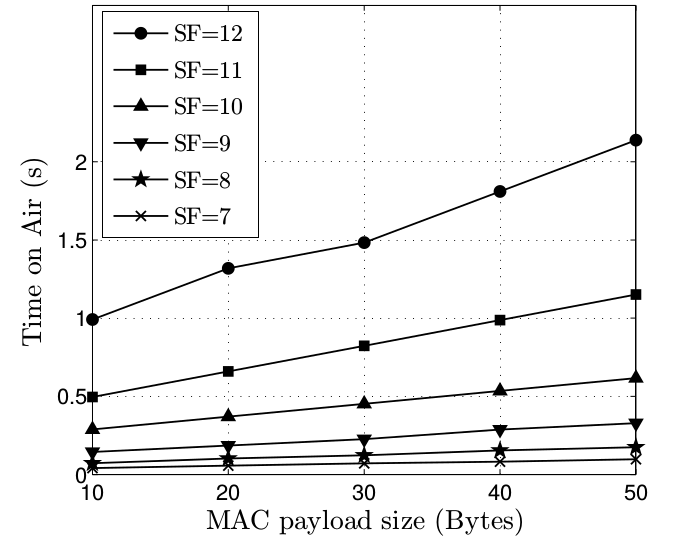
\includegraphics[scale=0.4]{images/estadoarte1.png}
\caption{Gráfica de tamaño de \textit{payload} MAC por tiempo que toma el paquete en llegar a destino. Fuente:\cite{Xavier}}
\label{arte:1}
\end{figure}
\begin{figure}[!ht]
\centering
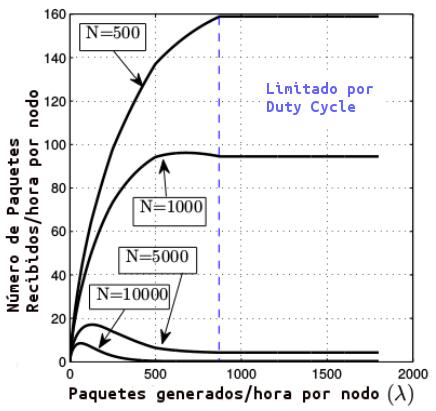
\includegraphics[scale=0.5]{images/estadoarte2.png}
\caption{Gráfica de paquetes generados en una hora por número de paquetes recibidos en una hora. Fuente:\cite{Xavier}}
\label{arte:2}
\end{figure}
Por otra parte, en otra investigación, se colocaron a prueba las capacidades de transmisión, pero en relación a la distancia máxima de transmisión, en zonas llanas sin interferencia por edificios o personas, y en zonas urbanas, con el objetivo de determinar si los LoRa cumplen con las especificaciones que entregan, y por otra parte, averiguar si pueden sobrepasar estas especificaciones técnicas entregadas por los fabricantes y descubrir nuevos límites para el uso de los dispositivos LoRa~\cite{Juha}.\\
En relación a las pruebas realizadas, el \textit{gateway} es situado a \SI{24}{\meter} sobre la altura del mar con una antena bi-cónica de \SI{2}{dbi} de ganancia, donde los nodos con los que se comunicará, uno estará navegando sobre un bote en un ambiente libre de edificios y árboles, mientras que el otro estará sobre el techo de un automóvil, donde cada nodo se alejará cada vez más sobre su medio de transporte, para evaluar si es posible transmitir efectivamente dentro de los parámetros que indican los fabricantes de LoRa, o si incluso es posible superar estas especificaciones. Los resultados obtenidos de las pruebas de medición de la investigación, pueden verse en las Tab~\ref{arte:3} y Tab~\ref{arte:4}~\cite{Juha}.\\
\begin{table}[!ht]
\centering
\begin{tabular}{|c|c|c|c|}
\hline
Rango & Número de            & Número de          & Porcentaje de  \\
      & paquetes trasmitidos & paquetes recibidos &  pérdida\\ 
      &                      &                    &   de paquetes \\ \hline
\si{0-2}{km} & \num{894} & \num{788} & \SI{12}{\percent} \\ \hline
\si{2-5}{km} & \num{1215} & \num{1030} & \SI{15}{\percent} \\ \hline
\si{5-10}{km} & \num{3898} & \num{2625} & \SI{33}{\percent} \\ \hline
\si{10-15}{km} & \num{932} & \num{238} & \SI{74}{\percent} \\ \hline
Total & \num{6813} & \num{4506} & \SI{34}{\percent} \\ \hline
\end{tabular}
\caption{Cantidad de paquetes transmitidos, recibidos y pérdida de paquetes por rango de distancia en medición hecha por nodo sobre auto. Fuente:\cite{Juha}}
\label{arte:3}
\end{table}

\begin{table}[!ht]
\centering
\begin{tabular}{|c|c|c|c|}
\hline
Rango & Número de            & Número de          & Porcentaje de  \\
      & paquetes trasmitidos & paquetes recibidos &  pérdida\\ 
      &                      &                    &   de paquetes \\ \hline
\si{5-15}{km} & \num{2998} & \num{2076} & \SI{31}{\percent} \\ \hline
\si{15-30}{km} & \num{690} & \num{430} & \SI{38}{\percent} \\ \hline
Total & \num{3688} & \num{2506} & \SI{32}{\percent} \\ \hline
\end{tabular}
\caption{Cantidad de paquetes transmitidos, recibidos y pérdida de paquetes por rango de distancia en medición hecha por nodo sobre bote. Fuente:\cite{Juha}}
\label{arte:4}
\end{table}
\newpage \noindent
Los resultados obtenidos a través de esta investigación, son de gran ayuda para el desarrollo de este proyecto, dado que entrega una guía de valores esperados al momento de realizar mediciones con los dispositivos reales~\cite{Juha}. Asimismo, otorga una guía de como se manifiestan parámetros como la tasa de errores en paquetes \gls{per}, para luego integrar al simulador con el fin de acercarlo más al funcionamiento real de los dispositivos. Y de la misma manera en la investigación que pone a prueba las capacidades de LoRa, entrega los conocimientos suficientes para poder modelar el comportamiento real de la saturación del canal en base a las retransmisiones de los nodos, y las colisiones generadas~\cite{Xavier}.
\section{Modelado de redes ALOHA}

El estándar \gls{lorawan} trabaja sobre la base del protocolo ALOHA, el cual es uno de los primeros protocolos de comunicación orientados a la conexión de dispositivos de forma inalámbrica. ALOHA trabaja sobre un canal de radio frecuencia, que utiliza tanto para el envío, como para la recepción de datos, por lo que para aumentar la transmisión efectiva de datos (\textit{throughput}), el protocolo ALOHA puro transmite datos en ventanas de tiempo aleatorias, y en caso de que el receptor no responda, en más del doble del tiempo que debiera responder con un acuse de recibo o \gls{ack}, el dispositivo emisor retransmitirá este paquete, y procederá con ese procedimiento hasta que reciba un acuse de recibo, con lo que concluye su transmisión de datos. Por otra parte Slotted ALOHA  o ``Ranurado'' implementa discretas ventanas de tiempo, donde el sólo podrá enviar o recibir datos, al inicio de una ventana de tiempo, con lo que se minimiza el número de colisiones~\cite{NORMAN}.\\
Slotted-ALOHA al ser un protocolo que permite las comunicaciones inalámbricas, con un buen manejo de colisiones, gracias a sus ventanas de tiempo discretas. Esta cualidad, llamó el interés de investigadores en generar ambientes virtuales, para simular el comportamiento de estos dispositivos, con el fin de poder realizar pruebas y estudios sobre el uso de este protocolo, sin necesidad de tener que instalar una red ALOHA con todos los costos asociados, tanto de tiempo como de dinero~\cite{Abdullah}.\\
En relación a los aportes del modelado de sistemas Slotted ALOHA, se realizan tres modelos que permiten el múltiple acceso de computadores mediante Slotted ALOHA, con el fin de otorgar modelos de simulación del protocolo para que estudiantes puedan comprender de mejor forma el cómo se comunican los dispositivos ALOHA~\cite{Abdullah}. Estos modelos de simulación imitan el comportamiento lógico del protocolo, entregando una herramienta útil para la comprensión del funcionamiento de redes de este tipo. Bajo este contexto, de la misma forma que nació la necesidad de modelar el funcionamiento del protocolo ALOHA. Adicionalmente se realizaron avances en el modelado de redes de sensores a gran escala, lo que entrega modelos que describen no sólo el funcionamiento del protocolo en condiciones ideales, si no que también la capacidad de modelar condiciones de borde y situaciones diferentes de las ideales, lo que acerca al módelo, a un comportamiento análogo al presente en los dispositivos reales~\cite{simulato}~\cite{simubook}.\\
Por otra parte, en una investigación se entrega un estudio sobre los diferentes simuladores de redes que existen, sus ventajas y desventajas frente al resto y los protocolos que acepta cada una de estas herramientas computacionales y sobre las capacidades de integración entre protocolos y tecnologías que ofrecen los distintos conjuntos de herramientas de simulación (\textit{frameworks})~\cite{Murat}.\\
En relación con este proyecto, todas las investigaciones mencionadas en este apartado, entregan la base teórica para el entendimiento del protocolo ALOHA, el cual es la base del funcionamiento de los dispositivos LoRa, y junto a esto hay investigaciones que entregan técnicas y métodos de cómo modelar tanto funcionamiento ideal y comportamiento lógico de protocolos en base a máquinas de estado ( en el caso de una simulación de eventos discretos), como también sobre el modelado de redes con parámetros como \gls{per}, atenuación de señal, entre otros elementos, que permiten el acercar un modelo de simulación, al comportamiento análogo de dispositivos reales~\cite{Abdullah}~\cite{simulato}. Cabe destacar que hay un artículo, que aporta con información sobre los diferentes \textit{frameworks} de simulación de redes, lo que permite tener una cantidad aceptable de información para poder decidir que software utilizar a la hora de desarrollar el simulador de dispositivos LoRa~\cite{Murat}.

\section{Integración de IoT en LoRaWAN}

%%tesis tomas, header compression y aplicaciones iot de lora%%
Los dispositivos LoRa, se comunican en base a transmisión de datos por radio frecuencia de un salto, esto junto con sistemas de modulación LoRa. En el escenario de enviar los datos obtenidos por los nodos LoRa con una aplicación web, el sistema no podría enviar los datos a través de Internet dado que no posee la capacidad de enrutamiento, no obstante el \textit{gateway} LoRa es capaz de realizar una retransmisión de los paquetes recibidos hacia un \textit{backend} (computador remoto) y con esto permitir la conectividad con aplicaciones web para la recepción de datos, aunque hasta el momento no es posible saber que nodo mandó un dato específico, o enviar datos desde el \textit{gateway} de forma directa hacia una dirección IP, esta carencia de los dispositivos LoRa limita las posibles aplicaciones con estos dispositivos. Bajo este contexto, algunos investigadores  han realizado modelos de compresión de cabeceras del protocolo IPv6 para dispositivos bajo el estándar \gls{lpwan}, donde se propone un modelo llamado 6LoWPAN que elimina ciertos campos de la cabecera del protocolo IPv6, de acuerdo a la configuración de los primeros \SI{16}{\bit}, con el fin de reducir el tamaño de la cabecera del paquete para direcciones IPv6 unicast, donde puede comprimirlos a \SI{512}{\bit} o \SI{128}{\bit} dependiendo de que campos se omiten, u omitir los campos opcionales por completo~\cite{lowpan}. En \cite{tomas}, este modelo teórico es aplicado a una red LoRa donde la cabecera IPv6 comprimida junto con el \textit{payload} deseado, se enviará a través del \textit{payload} de dispositivos \gls{lpwan} hacia el \textit{gateway}. Una vez llegado al \textit{gateway}, en este se construirá un paquete IPv6 con las especificaciones entregadas en la cabecera comprimida, donde adicionalmente se agregará la información relacionada al \textit{payload} del nodo emisor, y sus direcciones de red, las cuales al ser pertenecientes a una red LoRa, serán ingresadas en una tabla de enrutamiento que poseerá una equivalencia entre direcciones IPv6 y dirección de red LoRa, con el fin de poder luego enviar datos directamente desde los nodos hacia direcciones IPv6 y viceversa entregando la nueva función al \textit{gateway} LoRa de enrutador de mensajes.\newpage
\noindent
Cabe decir de que el \textit{gateway} LoRa para esta funcionalidad, necesita estar conectado al computador remoto que le provee de conexión a Internet, por medio de una interfaz virtual \gls{tun}, la que dejará pasar directamente los datos desde la red LoRa desde el \gls{tun} (donde está conectado el \textit{gateway} LoRa), hacia la salida a Internet del computador remoto. Si bien, la retransmisión de paquetes que posee nativa, realiza el mismo procedimiento, con la diferencia que ahora el \textit{gateway} LoRa creará el paquete de datos que se enviará, y este sólo será retransmitido hacia Internet, en cambio antes, el computador remoto tenía la labor de crear dicho paquete de datos, lo que entrega mayor autonomía e independencia de uso a los dispositivos LoRa.\\
Estos avances sobre la compresión de la cabecera IPv6 para dispositivos \gls{lpwan}, y la integración de IPv6 mediante el uso de estos modelos de compresión en una red LoRa, entregan a este proyecto el conocimiento necesario para poder diseñar un módulo que permita actuar de gestor de transición de una comunicación directa desde el \textit{gateway} hacia servicios locales dentro del computador remoto (sean bases de datos o aplicaciones web locales), y un intermediario mas seguro para la retransmisión de los paquetes, dado que al comunicarse directamente con la \gls{api} dentro del módulo bajo una conexión por \gls{socket}, entrega la posibilidad de realizar una conexión con un mayor nivel de seguridad, al tener la posibilidad de utilizar protocolos como TLS que dan la capacidad de cifrar la información y así evitar que un tercero atente contra la privacidad, integridad o disponibilidad de los datos.
\newpage
\section{Métodos de programación en C orientado a redes.}
%%libro de sockets, integracion de modulo%%
En muchas aplicaciones web, se han de utilizar scripts en sus servicios web para que realicen acciones deseadas por los desarrolladores, como también muchas veces son desarrollados scripts en el \textit{backend}, para realizar procedimientos como entrega de datos, creación de objetos, entre otros. El problema nace en que estos scripts son desarrollados en lenguajes como Python, Java o C, los que no tienen una orientación a red, si no, más bien a objetos, lo que dificulta el traspaso de datos obtenidos por los scripts hacia las aplicaciones web o sus servicios relacionados.\\
Bajo este contexto, nace la necesidad de que los scripts contenidos en aplicaciones web, se conecten tanto a \glspl{api} como a otros servicios existentes. Para poder llevar a cabo esta tarea, es necesario el uso de \glspl{socket}, los que constan de la apertura de conexiones bidireccionales a puertos determinados, que permiten la interacción en lectura como escritura contra servicios y aplicaciones web (Bases de datos, \glspl{api}, archivos de configuración, registros de depuración, etc). En el texto ``Programación en C orientada a redes'', enseñan múltiples técnicas, métodos y plantillas de código que permiten establecer conexión con servicios de red mediante el uso de \glspl{socket} en el lenguaje C~\cite{network}.\\
Los conocimientos aportados por este libro ayudaron en el desarrollo del módulo de transición de \gls{lorawan} a IPv6 en este proyecto, aportando métodos y funciones que otorgan la capacidad de conectar el \textit{gateway} LoRa con servicios y aplicaciones web. Esta conexión es generada en el mismo script que maneja la recepción de los mensajes de los nodos LoRa con el protocolo IPv6 integrado, resultando de esta forma, un sistema íntegro y con un nivel mayor de seguridad para poder conectar los datos obtenidos en la red LoRa con una aplicación web y todos sus servicios de red asociados.
\end{justify}
\chapter{Diseño y Definición de Modelo de Simulación}
\section{Definición de Variables y Parámetros}
Para el desarrollo del modelo de simulación es necesario acotar el sistema a simular a los objetivos deseados con esta simulación. Dado que el fin de esta simulación es simular el comportamiento físico de los dispositivos LoRa, algunos datos que en condiciones reales son variables serán tomadas como parámetros estáticos con el fin de simplificar el modelo de simulación. Los parámetros constantes de este sistema a modelar son los siguientes:
\begin{itemize}
\item coding rate$=4/5$
\item Ancho de Banda$=125KHz$
\item Packet Error Rate (PER)$=1\%$
\end{itemize}
Adicionalmente se han definido ciertos valores fijos para variables dependientes de los Spreading Factor a usar en la etapa de ADR de la comunicación LoRa(Véase Tab~\ref{par:1}).~\cite{orange}\\
\begin{table}[!ht]
\begin{tabular}{|c|c|c|c|}}
%&&&\\\hline
Spreading Factor & Bitrate & Alcance de Transmisión & Time on Air\\\hline
SF7 & $5470bps$ & $2km$ & $56ms$ \\\hline
SF8 & $3126bps$ & $4km$ & $100ms$ \\\hline
SF9 & $1760bps$ & $6km$ & $200ms$ \\\hline
SF10 & $980bps$ & $8km$ & $370ms$ \\\hline
SF11 & $440bps$ & $11km$ & $740ms$ \\\hline
SF12 & $290bps$ & $14km$ & $1400ms$ \\\hline
\end{tabular}
\label{par:1}
\caption{Asignación de Valores para los diferentes Spreading Factor}
\end{table}
\chapter{Pruebas y Resultados - Simulador de Dispositivos LoRa}
\section{Pruebas Realizadas}
\subsection{Parámetros y Variables en Mediciones}
\section{Resultados Obtenidos}
\subsection{Ajustes Planteados}
\subsection{Resultados Obtenidos luego de ajustes}
coming soon ;)
\chapter{Modulo de Transición LoRaWAN/IPv6}
\section{Funcionamiento}
\subsection{Contribuciones}
\subsection{Consideraciones}
coming soon ;)
\chapter{Pruebas de Verificación de Módulo de Transición LoRaWAN/IPv6}
\section{Elementos usados}
\section{Configuración de Pruebas}
\section{Resultados Obtenidos}
coming soon ;)
%%%%CONCLUSION%%%%%%
\begin{justify}
\chapter{Conclusiones}
En cuanto a el diseño e implementación del modelo de simulación desarrollados en este proyecto, se puede decir que la implementación del modelo de simulación, logra imitar de forma análoga el comportamiento de los dispositivos LoRa en relación a su funcionamiento lógico y físico, dado que logra simular cada fase de comunicación de los dispositivos LoRa, como la fase de emparejamiento, transmisión/retransmisión y la fase de descanso en nodos. De esta misma forma se imitó el funcionamiento físico de los dispositivos, lo que se pudo realizar implementando funciones que simulan de forma análoga el comportamiento de la tasa adaptativa de envío de datos. En las funciones que simulan el comportamiento del \gls{adr}, se analiza la distancia entre el nodo y el \textit{Gateway} de forma dinámica para asignar el canal (\gls{sf}) adecuado para dicha , cambiando con esto la tasa de envío de datos correspondiente al canal asignado. Adicionalmente se logró implementar una función que simula la pérdida de paquetes, donde en base a un \gls{per} asignado, esta función calcula si es necesario o no descartar un paquete en cada canal para cumplir con el \gls{per} asignado.\\
La implementación de este modelo de simulación muestra el cómo se realiza la comunicación de los dispositivos LoRa en una red de topología estrella, donde es posible probar tanto distribuciones de nodos en los distintos canales o \gls{sf}, como también el rendimiento de los dispositivos al agregarle variables reales como el porcentaje de la pérdida de paquetes, o la asignación dinámica de la tasa de envío, tomando la distancia que posee el nodo hasta el \textit{Gateway}.\\
En la implementación del módulo de transición LoRaWAN/IPv6, se logró la correcta adquisición de la información, tanto de los dispositivos de la red LoRa, como del \textit{Payload} que se busca transmitir hacia un servicio de carácter web como lo es una Base de datos. Dado que este módulo de transición es implementado en base al uso de \glspl{socket}, es posible agregar, dependiendo de las necesidades del desarrollador, una capa de cifrado a los datos usando OpenSSL u TLS para comunicarse con los servidores objetivo, donde en el caso de agregar cifrado, se estaría además añadiendo una capa de seguridad adicional a la existente actualmente (cifrado sobre el mensaje), al usar el método de retransmisión de paquetes hacia el computador remoto, el cual sólo realiza una condición \textit{Pass Through} en el \textit{Firewall} local.\\
\noindent
En relación al desarrollo del modelo de simulación, este se caracteriza por aportar la capacidad de realizar pruebas de conectividad de dispositivos LoRa, con distintas distribuciones y con diferentes configuraciones de parámetros (\gls{per}, tasa de envío de datos, etc.) en un ambiente virtual, obteniendo resultados análogos a los que se obtendrían con una medición en un ambiente real. No obstante, la topología abarcada en este proyecto es la topología estrella, este modelo no admite distribuciones estrella-de-estrellas ni variantes más complejas, por lo que este aporte iría enfocado en redes simples con un \textit{Gateway} único en la red.\\
En cuanto al módulo de transición, este otorga la capacidad de poder interconectar de forma directa una red LoRa con un servicio de red, teniendo la posibilidad de agregar o no, una capa de seguridad extra al canal de transmisión hacia Internet.
\end{justify}
%\input{cha-dos}
% ... mas archivos de capitulos
%
% ---------------------------------------------------------------
% Bibliograf�a
% ---------------------------------------------------------------
% tubiblio.bib es el archivo con la base de datos bibliografica
%
\putbibliography{tubiblio}

%
% ---------------------------------------------------------------
% Simbolog�a y glosario
% ---------------------------------------------------------------
% simbolos.tex es el archivo de simbolos (y glosario)
%
%\begin{symbology}
%\input{simbolos}  % archivo propio de simbolos
%\end{symbology}
%
% ---------------------------------------------------------------
% Anexos
% ---------------------------------------------------------------
\appendix
%
% aca se incluyen los archivos con el texto de los anexos
% (Ej.: anx-uno.tex es el archivo de un anexo)
%

%\input{anx-uno}
%\input{anx-dos}
% ... mas archivos de anexos
%
% ---------------------------------------------------------------
% Fin del documento
% NO ESCRIBIR DESPU�S DE ESTA LINEA
\backmatter
\end{document}
% ---------------------------------------------------------------
